\documentclass[12pt]{article}

\usepackage[danish]{babel}
\usepackage[utf8]{inputenc}
\usepackage{amsmath}
\usepackage{pbox}
\usepackage{graphicx}

\begin{document}

% !TEX root = ../rapport.tex

\begin{titlepage}
	\centering
	\includegraphics[width=1\textwidth]{kapitler/billeder/lowrider.jpg}
	\vspace{1cm}
	{\scshape\Large Semesterprojekt\par}
	\vspace{1.5cm}
	{\huge\bfseries Poleposition\par}
	\vspace{2cm}
	{\Large\itshape Alexander D. Larsen, Frederik N. Larsen, Mikkel L. Olsen, Phillip M. Kyndbøl og Rasmus Haugaard\par}
	\vfill
	Faglig vejleder\par
	\textsc{Jan Petersen}

	\vfill

% Bottom of the page
	{\large 08/02 - 25/05 2016}
\end{titlepage}


\tableofcontents

\newpage

\section*{Resumé}
Denne rapport beskriver udviklingen af en selvkørende scalextric bil. Bilen bliver udviklet til at kunne køre selv på en ukendt bane. For at kunne netop dette udvikles et mapning-system til at registrere den ukendte bane. Mapningen bliver lavet vha. et digitalt gyroskop og en omdrejningstæller på motoren. Et motorstyringsprogram udvikles til at bruge mapningen. Der udvikles også en elektromagnet til at skabe downforce på bilen, og en stregdetektor til at registrere startlinjen på banen. Der bliver udviklet et 3D-printet chassis for at få plads til alle justeringerne i bilen. Alle de ting der bliver udviklet til bilen er med henblik på at sætte den hurtigst mulige omgangstid på den ukendte bane. 


% !TEX root = ../rapport.tex
\section{Indledning}

SKRIV INDLEDNING

\newpage

% !TEX root = ../rapport.tex

\section{Problemformulering}

Projektet har til formål at udvikle en mikrocontroller-baseret styring til en racerbil med henblik på at opnå den hurtigste omgangstid på en ukendt bane.
Der vil blive fokuseret på to hovedområder; Den fysiske del samt softwaren. Den fysiske del består af optimering af tophastighed, acceleration, bremselængde og hastighed i sving.
Softwaren skal kunne kortlægge den ukendte bane og styrer bilens motor derefter på baggrund af data fra sensorer.

\begin{itemize}
	\item Design en elektromagnet til at skabe downforce til optimering af svinghastighed og optimering af bremselængde.
	\item Undersøg effekten af fysiske ændringer på bilen f.eks. fastsættelse af affjedring i fht. til optimering af banetider.
	\item Design et optoelektronisk system, der kan registrere en startlinje.
	\item Design en optoelektronisk system, der kan registrere motoromdrejninger.
	\item Udvikle et program, der kortlægger en ukendt bane på baggrund af data fra sensorer.
	\item Udvikle et motorstyringsprogram, der optimerer omgangstiden på baggrund af kortlægningen samt data fra sensorer.
\end{itemize}



% !TEX root = ../rapport.tex

\newpage
\section{Idégenerering}
For at opnå den hurtigste omgangstid skal der være en kombination af den rigtige fysiske opsætning af bilen og en mikrocontroller der fortæller bilen hvordan den skal køre på banen.
Det første der blev undersøgt var de fysiske optimeringer der kunne laves på bilen.

\subsection{Hardware}

\begin{itemize}
\item Forøgelse af acceleration og tophastighed
\item Formindskelse af bremselængde
\item Optimering hastighed igennem sving
\end{itemize}
For at optimere ovenstående er der flere ting der kan overvejes, se figur \ref{fig:mindmap1}.

\begin{figure}[ht]
    \centering
    \includegraphics[width=1\textwidth]{kapitler/billeder/Mindmap1.jpg}
    \caption{Idégenerering til optimering af omgangstid}
    \label{fig:mindmap1}
\end{figure}



\subsection{Software}
Udover de fysiske komponenter i bilen skal bilens omgangstid også optimeres ved hjælp af software.


\begin{figure}[ht]
    \centering
    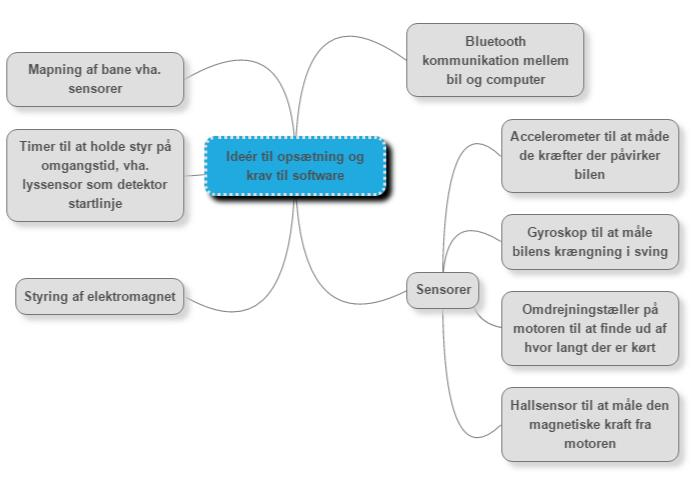
\includegraphics[width=0.8\textwidth]{kapitler/billeder/Mindmap2.jpg}
    \caption{Idégenerering til opsætning af software}
    \label{fig:mindmap2}
\end{figure}


Idéen er, at software skal kunne kortlægge den ukendte bane ved hjælp af sensorer, ved først at kører et par omgange.
Når banen er blevet kortlagt og gemt i bilens hukommelse kan den sætte en hurtig omgangs tid.
Mikrocontrolleren ved herefter, hvor og hvornår der er et sving, hvor der skal bremse og hvor hårdt den kan accelerere de forskellige steder på banen.
Idéen er altså, at bilen skal optimeres til at køre en så hurtig omgangstid som muligt, ved både at optimere det fysiske på bilen, dens hardware og software.

% !TEX root = ../rapport.tex
\subsection{Fysiske modifikationer}

For at minimere vægten af bilen er alt unødvendigt plastik blevet fjernet fra bilen. Grunden til dette kan beskrives vha. Newtons 2. lov. Bilen bevæger sig fremad med en kraft F, og bilen har en masse m. 
\begin{equation}
F=m \cdot a
\end{equation}
\begin{equation}
a = \frac{F}{m}
\end{equation}
Accelerationen a, stiger derved jo mindre massen af bilen er. 

Downforce er ekstremt brugbart i sving da det hjælper med at holde bilen på banen ved højere fart. Downforce er mindre brugbart på lige strækninger da bilen let bliver på banen og downforce faktisk vil sænke bilens acceleration og topfart. Derfor indføres der justerbar downforce med elektromagneten. I det 3D-printet chassis er der en indbygget holder til elektromagneten. Elektromagnet er placeret bagerst for at give kontra til den permamagnet der i forvejen sidder i bilen. Permamagneten er placeret foran og tæt på splitten for at trække splitten ned i banen. For uddybning af elektromagneten se sektion \ref{Elektromagnet}.

\subsubsection{3D-printet chassis}

For at kunne hurtigt gennem sving kræver det et lavt tyngdepunkt i bilen, jo lavere tyngdepunktet er jo hurtigere kan bilen klare at køre gennem et sving uden at kæntre. Dette fænomen kan ses på figur \ref{fig:bilsving} nedenfor.
\begin{figure}[ht]
    \centering
    \includegraphics[width=0.8\linewidth]{kapitler/billeder/bilsving.png}
    \caption{Skitse af bilen i et venstresving med to forskellige tyngdepunkter}
    \label{fig:bilsving}
\end{figure}
På bil 1 er tyngdepunktet (den blå prik) lavt og derved har den en kortere arm (den grønne streg) fra tyngdepunktet til omdrejningspunktet (den røde prik). Omdrejningsmomentet(den lilla pil) kan beskrives som:
\begin{equation}
\tau = F \cdot L
\end{equation}
Hvor $\tau$ er omdrejningsmomentet, L er armen (den grønne streg) og F er kraften der påvirker den (den sorte pil). Der antages at der skal det samme omdrejningsmoment ($\tau$) til at bilen kæntre.
\begin{equation}
F = \frac{\tau}{L}
\end{equation}
Derved kan det ses at når armen, L, bliver større skal der mindre kraft F til bilen kæntre. 
Ved at fjerne affjedringen optimeres tyngdepunktet også da karrosseriet er i sin laveste tilstand hele tiden, og ikke kun når fjedrene er trykket sammen.

Det udleveret chassis på racerbilen er meget vakkelvornt, og kan vrides let. For at optimere dette er der blevet 3D-printet et nyt forstærket chassis. Det chassis er stærkere end det gamle og giver lettere plads til at montere sensorer og aktuatore i bilen. Det nye chassis er tegnet i AutoDesk Inventor og derefter 3D-printet med Makerbot. 3D-printet er printet i flere dele og derefter samlet med skruer. En fordel ved at printet er i flere dele er hvis én del går i stykker skal man ikke printe det hele igen. 3D-tegningen ses på figur \ref{fig:3Dtegning} nedenfor.

\begin{figure}[ht]
    \centering
    \includegraphics[width=0.7\textwidth]{kapitler/billeder/3Dtegning.jpg}
    \caption{3D-tegning af bilens chassis}
    \label{fig:3Dtegning}
\end{figure}


Det vil sige at den affjedring der følger med bilen er blevet fjernet og erstattet med det afstivet chassis. Grunden til man har affjedring i virkelige biler er for at beskytte både kører og motor, da man aldrig er sikker på asfaltens tilstand. Da banen racerbilen skal køre på er flad og der er ingen kører der skal beskyttes, vil det optimere bilens hastighed igennem sving uden at den kæntre, at fjerne affjedringen. På figur \ref{fig:racerchassis} nedenfor ses det 3D-printet chassis med motor og hjul på.

\begin{figure}[ht]
    \centering
    \includegraphics[width=0.7\textwidth]{kapitler/billeder/racerchassis.jpg}
    \caption{3D-printet chassis med motor og hjulakser}
    \label{fig:racerchassis}
\end{figure}

Det nye 3D-printet chassis er også udviklet til at ATmega-boardet kan skrues direkte på. Det nye chassis er blevet testet mod det gamle chassis i et 180 graders sving. Med det gamle chassis var den maksimale indgangshastighed bilen kunne køre ind i et sving uden at ryge af 1.9 m/s. Med det nye chassis kan bilen kører samme sving med en indgangshastighed på 2.6 m/s uden at ryge af.

% !TEX root = ../rapport.tex
\newpage
\subsection{I2C kommunikation}
Til at kommunikere med de digitale komponenter, herunder vores udleveret accelerometer og gyroskop, anvendes den kommunikationsprotokol kaldet I2C eller TWI (”two-wire interface”). Navnet ”two-wire interface” kommer af, at hele kommunikationen foregår over kun 2 ledninger, men hvor der samtidig er mulighed for at kommunikere med mange komponenter.

\begin{figure}[ht]
    \centering
    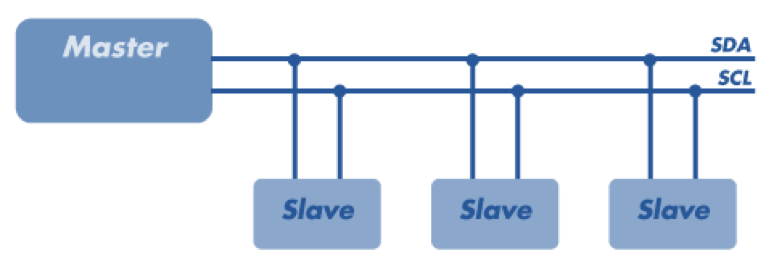
\includegraphics[width=0.8\textwidth]{kapitler/billeder/i2c-princip.png}
    \caption{Viser en skitse af hvordan opsætningen kan laves mellem
én ”master” og flere ”slaver”, kun ved brug af to forbindelser.}
    \label{fig:i2cprincip}
\end{figure}

De to forbindelser der bruges til vores TWI kommunikation hedder SCL (”Serial Clock Line”) og SDA (”Serial Data Line”). SCL er en clock der sættes af master, for at både master og slaven snakker og lytter ved en fælles frekvens. SDA er den forbindelse, hvor alt data bliver overført både fra slaven til master, men også fra master til slaven. Denne form for kommunikation kaldes for halv-duplex, og fungere ligesom en walkie talkie, hvor der kun er én der snakker af gangen, imens den anden lytter.

\subsubsection{Kommunikationsprotokol}

Kommunikationen mellem master og slave, foregår ud fra en bestemt protokol, som er opgivet ved den enkelte slaves datablad. Denne protokol er den samme for accelerometeret og gyroskopet, og er illustreret på figur \ref{fig:i2conebyte}. 

\begin{figure}[ht]
    \centering
    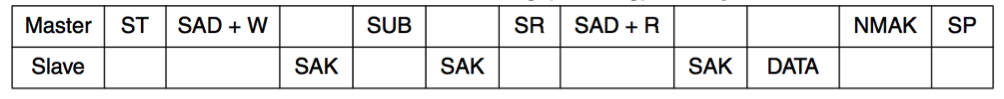
\includegraphics[width=1\textwidth]{kapitler/billeder/i2c-onebyte.png}
    \caption{Kommunikationsprotokol for gyroskopet via I2C}
    \label{fig:i2conebyte}
\end{figure}

Figur \ref{fig:i2conebyte} viser skridt for skridt, hvordan kommunikationsprotokollen er opbygget, hvis man vil læse data én gang fra én af vores to digital komponenter.

Protokollen indeholder følgende instruktioner for at modtage én data byte:

\begin{enumerate}
\item ST (”Start Bit”): Master sender et start bit til alle slaverne, for at starte kommunikationen.
\item SAD+W (”Slave Adress + Write”): Master sender en slave adresse på 7 bits, og det sidste bit beskriver om der skal læses eller skrives, i dette tilfælde skal der skrives. Adressen er specifik for hver komponent og fortæller hvilken slave, som resten af kommunikationen kommer til at foregå med. Det sidste bit indikere, at masteren vil skrive noget til slaven.
\item SAK (”Slave Acknowledge”): Slaven med den valgte adresse sender er ACK bit tilbage, som fortæller at den har hørt hvad masteren sagde, og gør klar til at læse næste instruktions.
\item SUB (”Sub adress”): Master sender herefter en underadresse. Denne underadresse er en 7 bit adresse, som fortæller hvilken register inde i den valgte komponent, der gerne vil adresseres.
\item SAK (”Slave Acknowledge”): Slaven sender endnu et SAK bit, og gør klar til næste instruktion.
\item SR (”Repeated Start”): Master sender herefter et gentagende start bit. Der skal altid sendes en start/repeated start instruktion, hver gang der skiftes mellem at læse eller skrive. Ved repeated start vedholdes forbindelsen til slaven, og slaven ved derfor allerede hvilken underadresse, der herefter skal læses fra.
\item SAD+R (”Slave Adresse + Read”): Master sender herefter igen slave adressen, samt én read bit, for at ændre at vi nu gerne vil læse på slaven, modsat at vores tidligere write, som skrev til slaven.
\item SAK (”Slave Acknowledge”):  Slaven sender en ACK bit.
\item DATA (”Data Byte”): Slaven sender efterfølgende en data byte til master.
\item NMAK (”Master Not Acknowledge”): Herefter sendes én NMAK fra master til slaven, for at indikere at der ikke skal læses mere data.
\item SP (”Stop Bit”): Til sidst sender master et stop bit, for at afslutte kommunikationen.
\end{enumerate}

% !TEX root = ../rapport.tex
\newpage
\subsection{Boost converter}
En boost converter er et analogt DC-DC kredsløb som har en højere udgangsspænding end indgangsspænding.
Idéen med en boost converter er at øge effekten hen over motoren og derved få højere acceleration og tophastighed. Ved 15V trækker motoren kun 0,5A og derved bruger den kun 7.5 Watt. Da vi har en strømforsyning der kan levere 30 Watt kan vi udnytte det meget mere ved at øge spændingen. Dette vil dog gøre vi ikke helt kan trække 30 Watt da man aldrig kan lave en 100 procent effektiv boost converter.  Ideén er at have en udgangsspænding på 30V, og hvis boost converteren kun er 85 procent effektiv giver det en strøm, I på:
\begin{equation}
15V \cdot 2A = 30 W
\end{equation}
\begin{equation}
30 W \cdot 0,85 = 25,5 W
\end{equation}
\begin{equation}
I = \frac{25,5 W}{30 V} = 0,85A
\end{equation}
Hvilket burde være mere end rigeligt til at drive motoren langt hurtigere end med 15V og 0,5A

\begin{figure}[ht]
    \centering
    \includegraphics[width=0.8\linewidth]{kapitler/billeder/BoostConverter.png}
    \caption{Skematisk tegning af en boost-converter}
    \label{fig:boostconvert}
\end{figure}

På figur \ref{fig:boostconvert} ses et forsimplet kredsløb af en boost converter. Idéen er at når switchen S, sluttes bliver der en magnetisk kraft opladet i spolen L. Når switchen bliver brudt vil kraften fra spolen oplade kondensatoren, men da strømmen i en spole ikke kan ændres momentant vil der også løbe strøm fra spændingskilden igennem spolen og derved vil der opnås en højere spænding over kondensatoren C.

Da dette kredsløb gerne skulle være selvkørende bruges der ikke en switch, men en MOSFET som skal aktiveres af et højfrekvent signal. Det er vigtig at frekvensen er så høj at spolen ikke når at gå i mætning, som vil sige at det ikke når det punkt hvor virker som en kortslutning, da kredsløbet så ville være en direkte kortslutning fra vores spændingskilde til ground.

Det er vigtigt at udvælge de rigtige komponenter til dette kredsløb da det er et højfrekvent kredsløb hvor der løber store strømme. En schottky-diode benyttes da den kan switche ved langt højere frekvenser end en almindelig diode og har et lavere spændingstab henover den og dermed får vi større effektivitet. Kondensator skal have så stor kapitans som mulig(selvfølgelig inden for rimelighedens grænser) og kunne tåle høje spændinger hen over den. MOSFET'en som bliver brugt som switch skal kunne switche hurtigt og kunne klare at der løber stor strøm igennem den uden at blive alt for varm.

En af de problemer ved at bygge en boost converter som fast skal kunne levere 30V er an på motorens hastighed ændre motorens indre modstand sig, og derved ændrer spændingen sig også. Det er derfor nødvendigt at have en form for feedback der fortæller frekvensgeneratoren om den skal øge eller sinke frekvensen for at outputtet bliver som forventet. Der findes IC-kredse der gør dette automatisk, men da gruppen ikke kan stå indenfor hvordan de IC-kredse virker er der blevet valgt ikke at bruge dem i  bilen, og derved ville det blive for stor en udfordring at bygge boost converteren i forhold til den tid der var til projektet.  

% !TEX root = ../rapport.tex
\newpage
\section{Lap timer}
Formålet med Lap timeren er at have et stykke kode som måler og returnere omgangstiden, for hver omgang bilen køre. Lap timeren er baseret på "timer1" og er derfor den største timer. Lap timeren bliver udover omgangstid, også brugt af andre kode moduler, til at tage tid.
\subsection{Opsætning af Lap timer}
\subsection{Kode}
\subsection{Macro's}

* Valg af prescaler (udregninger)\\
	-præcision
	-maks/min omgangs tider 
	
* 24-bit register\\
% !TEX root = ../rapport.tex
\newpage

\section{Motor omdrejninger (kode)}
% !TEX root = ../rapport.tex


\section{Konklusion}


Mikkel skriv noget om elektromagnet her


Det optoelektriske system der blev udviklet til at detektere startlinjen virker optimalt og giver et klart signal gennem schmitt-triggeren. Det samme med motor omdrejningstælleren der også virker optimalt og giver en klar høj-lav puls når motoren kører, og derved en klar indikation om hvor langt bilen har kørt.
Kortlægning af banen er blevet udviklet, for at kunne beregne den bedst mulige omgangstid for bilen.
Denne kortlægning bliver gemt som segmenter i SRAM, for efterfølgende at kunne bliver behandlet.
Ved brug af bane segmenterne og sensorerne styre kortlæsnings modulet: elektromagneten, H-broen og hastigheden. Koden virker som forventet, med maksimal acceleration på lige stykker og samtidig nedbremsning op til sving.
De fysiske ændringer der er blevet fortaget har stor effekt på bilen. Specielt det nedsatte tyngdepunkt, det afstivet chassis og placering af magneter gør at bilen kan tage sving meget hurtigere uden at kæntre.

Samlet giver alle ændringerne at bilen kan kører på ukendt bane, og lave et optimalt forsøg på en hurtig omgangstid.




% !TEX root = ../rapport.tex
\section{Bilag-lap-timer}
\begin{figure}
\centering
\includegraphics[width=0.4\textwidth]{kapitler/billeder/lapt/lapt-flow.png}
\caption{Flowchart over første rutine i lap-timer}
\label{fig:lapt-flow}
\end{figure}


\end{document}
